\documentclass[3p,preprint,number]{elsarticle}
\DeclareGraphicsExtensions{.pdf,.gif,.jpg,.pgf}
\usepackage{colortbl}
\usepackage{tikz}
\usepackage{pgfplots}
\usepackage{amsmath}
\pgfplotsset{compat=1.17}
\usepackage{amssymb}
\usepackage{xcolor}
\usepackage[latin1]{inputenc}
\usetikzlibrary{patterns}
\usepackage{tikz}
\usetikzlibrary{matrix}

\begin{document}

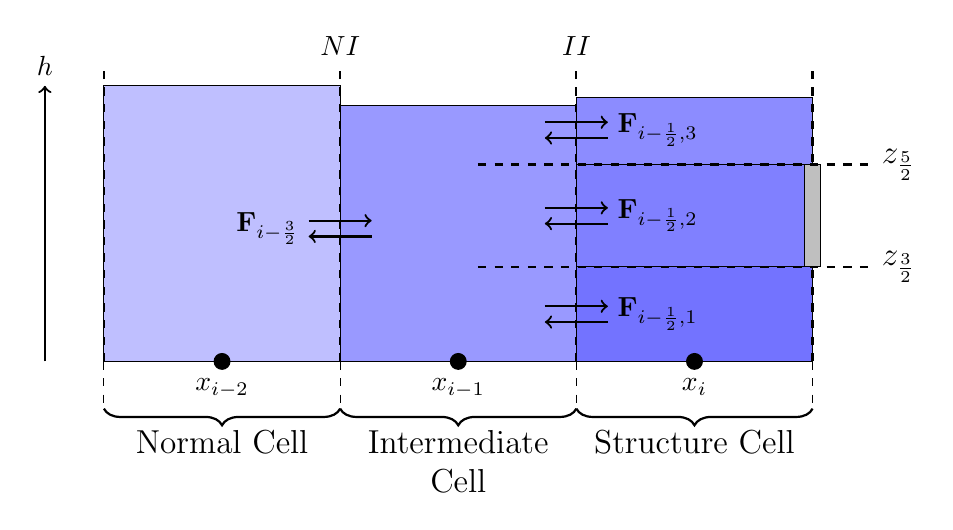
\begin{tikzpicture}
				\draw[thick, ->] (-0.75,0) -- (-0.75,3.5) node[above] {$h$};
				\fill[fill=blue!25!white, draw=black] (0,0) rectangle (3,3.5); %normal cell
				\fill[fill=blue!40!white, draw=black] (3,0) rectangle (6,3.25); %intermediate cell
				\fill[fill=blue!55!white, draw=black] (6,0) rectangle (9,1.2); %structure cell 1
				\fill[fill=blue!50!white, draw=black] (6,1.2) rectangle (9,2.5); %structure cell 2
				\fill[fill=blue!45!white, draw=black] (6,2.5) rectangle (9,3.35); %structure cell 3
				\draw[thick, dashed] (0,0) -- (0,3.75);%interface
				\draw[thick, dashed] (3,0) -- (3,3.75) node[above] {$NI$};%interface
				\draw[thick, dashed] (6,0) -- (6,3.75) node[above] {$II$};%interface
				\draw[thick, dashed] (9,0) -- (9,3.75);%interface
				\fill[fill=black!25!white, draw=black] (8.9,1.2) rectangle (9.1,2.5); %Structure Interface
				\draw[thick, dashed] (4.75, 1.2) -- (9.75, 1.2) node[right] {\large$z_{\frac{3}{2}}$};
				\draw[thick, dashed] (4.75, 2.5) -- (9.75, 2.5) node[right] {\large$z_{\frac{5}{2}}$};
				
				\draw[->, thick] (2.6,1.7875) -- (3.4,1.7875); %fluxes
				\draw[->, thick] (3.4,1.5875) -- (2.6,1.5875); %fluxes
				\node[left] at (2.6, 1.6875) {$\textbf{F}_{i-\frac{3}{2}}$};
				\draw[->, thick] (5.6,0.7) -- (6.4,0.7); %fluxes
				\draw[->, thick] (6.4,0.5) -- (5.6,0.5); %fluxes
				\node[right] at (6.4, 0.6) {$\textbf{F}_{i-\frac{1}{2},1}$};
				\draw[->, thick] (5.6,1.95) -- (6.4,1.95); %fluxes
				\draw[->, thick] (6.4,1.75) -- (5.6,1.75); %fluxes
				\node[right] at (6.4, 1.85) {$\textbf{F}_{i-\frac{1}{2},2}$};
				\draw[->, thick] (5.6,3.0375) -- (6.4,3.0375); %fluxes
				\draw[->, thick] (6.4,2.8375) -- (5.6,2.8375); %fluxes
				\node[right] at (6.4, 2.9375) {$\textbf{F}_{i-\frac{1}{2},3}$};
				\draw [decorate, decoration={brace,amplitude=6pt,raise=0pt}, thick] (9,-0.6) -- (6,-0.6); %Curly bracket
				\node[below] at (7.5,-0.75) {\large Structure Cell};
				\draw [decorate, decoration={brace,amplitude=6pt,raise=0pt}, thick] (6,-0.6) -- (3,-0.6); %Curly bracket
				\node[below] at (4.5,-0.75) {\large Intermediate};
				\node[below] at (4.5,-1.25) {\large Cell};
				\draw [decorate, decoration={brace,amplitude=6pt,raise=0pt}, thick] (3,-0.6) -- (0,-0.6); %Curly bracket
				\node[below] at (1.5,-0.75) {\large Normal Cell};
				\draw[dashed] (0,0) -- (0,-0.6);
				\fill[fill=black, draw=black] (1.5,0) circle (0.1cm);
				\node[below] at (1.5,-0.1) {$x_{i-2}$};
				\draw[dashed] (3,0) -- (3,-0.6);
				\fill[fill=black, draw=black] (4.5,0) circle (0.1cm);
				\node[below] at (4.5,-0.1) {$x_{i-1}$};
				\draw[dashed] (6,0) -- (6,-0.6);
				\fill[fill=black, draw=black] (7.5,0) circle (0.1cm);
				\node[below] at (7.5,-0.1) {$x_{i}$};
				\draw[dashed] (9,0) -- (9,-0.6);
			\end{tikzpicture}

\end{document}